\documentclass[a4paper]{article}
\usepackage[utf8]{inputenc}
\usepackage[spanish, es-tabla, es-noshorthands]{babel}
\usepackage[table,xcdraw]{xcolor}
\usepackage[a4paper, footnotesep = 1cm, width=20cm, top=2.5cm, height=25cm, textwidth=18cm, textheight=25cm]{geometry}
%\geometry{showframe}

\usepackage{tikz}
\usepackage{amsmath}
\usepackage{amsfonts}
\usepackage{amssymb}
\usepackage{float}
\usepackage{graphicx}
\usepackage{caption}
\usepackage{subcaption}
\usepackage{multicol}
\usepackage{multirow}
\setlength{\doublerulesep}{\arrayrulewidth}
\usepackage{booktabs}

\usepackage{hyperref}
\hypersetup{
    colorlinks=true,
    linkcolor=blue,
    filecolor=magenta,      
    urlcolor=blue,
    citecolor=blue,    
}

\newcommand{\quotes}[1]{``#1''}
\usepackage{array}
\newcolumntype{C}[1]{>{\centering\let\newline\\\arraybackslash\hspace{0pt}}m{#1}}
\usepackage[american]{circuitikz}
\usetikzlibrary{calc}
\usepackage{fancyhdr}
\usepackage{units} 

\graphicspath{{../Ejercicio-1/}{../Ejercicio-2/}{../Ejercicio-3/}{../Ejercicio-4/}}

\pagestyle{fancy}
\fancyhf{}
\lhead{22.01 Teoría de Circuitos}
\rhead{Mechoulam, Lambertucci, Rodriguez Turco, Londero, Galdeman}
\rfoot{\centering \thepage}
\begin{document}

\subsection{Introducción}

En esta sección se implementó un filtro High-Pass utilizando una aproximación \textbf{Cauer} e implementandola con celdas \textbf{Sedra}, el filtro a diseñar deberá cumplir con la siguiente plantilla.
\begin{table}[H]
\centering
\begin{tabular}{|c|c|}
\hline
$f_s$      & 11.65kHz          \\ \hline
$f_p$      & 23.3kHz           \\ \hline
$A_p$      & 2dB               \\ \hline
$A_s$      & 40dB              \\ \hline
$|Z_{in}|$ & $\geq 50k \Omega$ \\ \hline
\end{tabular}
\end{table}
\subsection{Aproximación de Cauer.}
Para esta sección se utlizó la aproximación elíptica de \textbf{Cauer}, además se propuso una plantilla mas restrictiva, con el fin de asegurar el cumplimiento de la original, siendo esta la plantilla final.
\begin{table}[H]
\centering
\begin{tabular}{|c|c|}
\hline
$f_s$      & 11.65kHz          \\ \hline
$f_p$      & 23.3kHz           \\ \hline
$A_p$      & 1dB               \\ \hline
$A_s$      & 45dB              \\ \hline
$|Z_{in}|$ & $\geq 50k \Omega$ \\ \hline
\end{tabular}
\end{table}
Obteniendo la siguiente función transferencia, expresandola como producto de transferencias de segundo orden:
\begin{align}
	H(s)=\frac{ {s}^{2}+ 124088460.2 
 }{s^2+s\cdot 5466 + 519.84\cdot 10^6 } \cdot \frac{  {s}^{2}+
 23794591.32 }{s^2+s\cdot 48182 + 1.6\cdot 10^9 }
\label{eq:trans}
\end{align}
Y el siguiente diagrama de polos y ceros:
\begin{figure}[H]
	\centering
	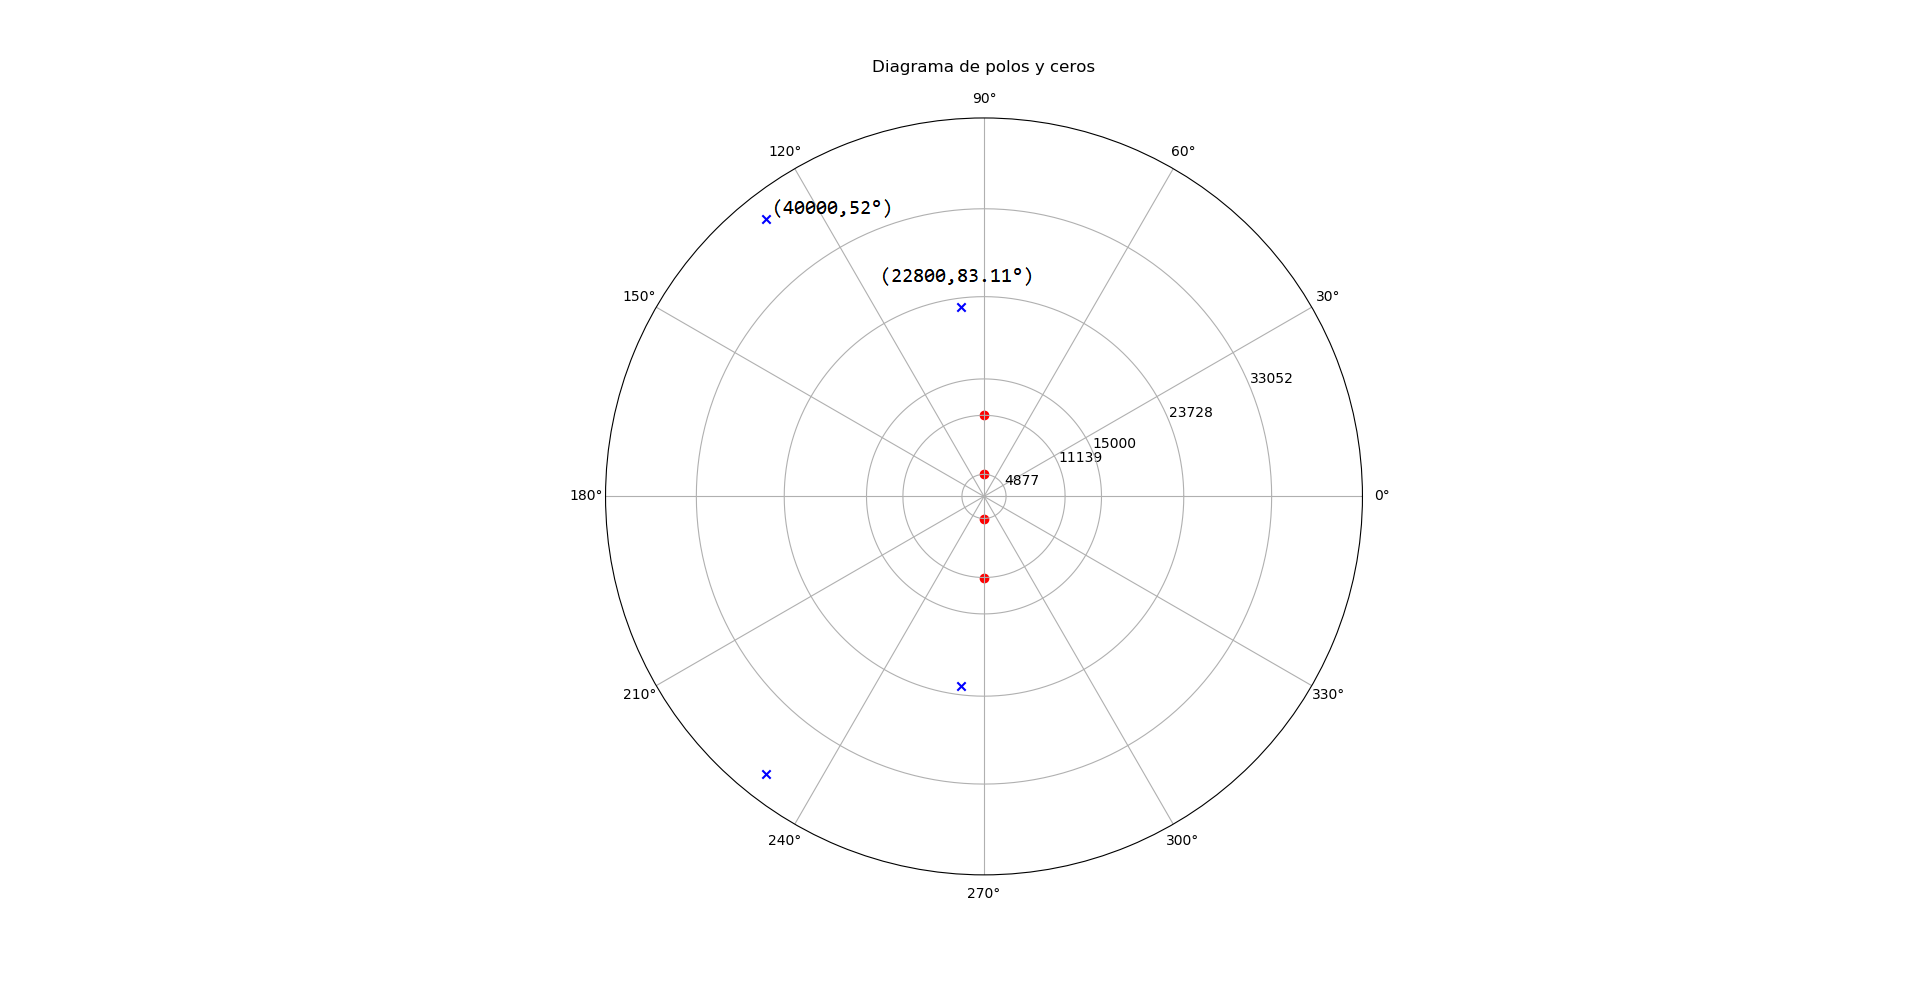
\includegraphics[width=\textwidth]{Imagenes-Ej3/DiagramaPolosYCeros.png}
	\label{fig:poleZeroDiag}
	\caption{Diagrama Polos y Ceros}
\end{figure}

Teniendo los pares de polos con un Q de 0.84 la primer etapa y 4.17.


Finalmente se graficó la respuesta en frecuencia tanto en fase como en módulo:
\begin{figure}[H]
	\centering
	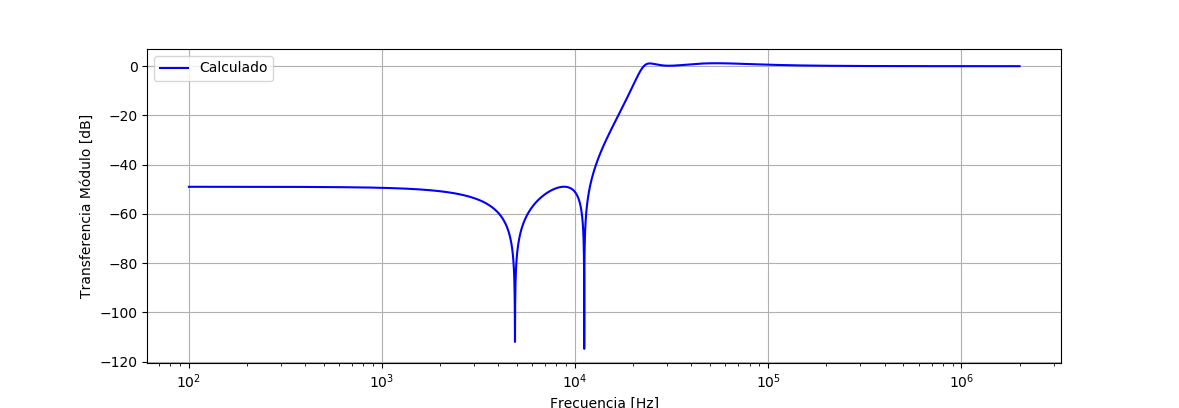
\includegraphics[width=\textwidth]{Imagenes-Ej3/BodeCalc.png}
	\label{fig:Bodecalc}
	\caption{Diagrama de bode Módulo}
\end{figure}

\begin{figure}[H]
	\centering
	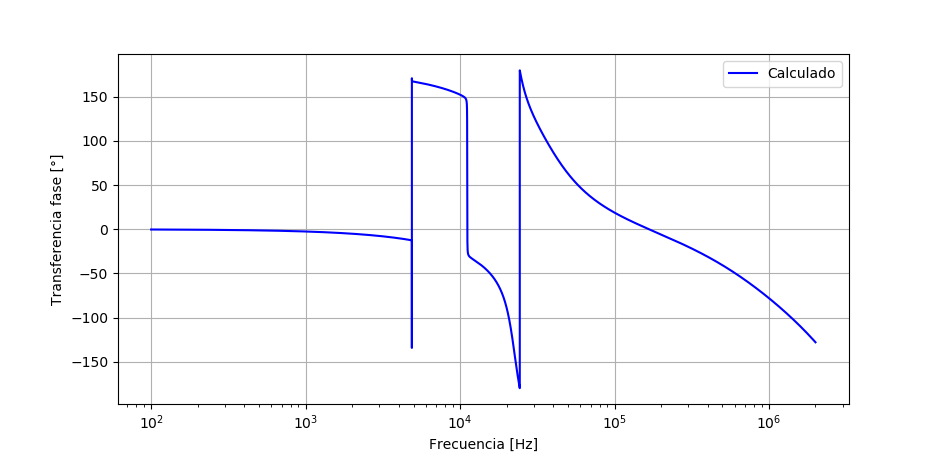
\includegraphics[width=\textwidth]{Imagenes-Ej3/BodeFaseCalc.png}
	\label{fig:BodeCalcF}
	\caption{Diagrama de bode Fase}
\end{figure}
\subsubsection{Elecciones de diseño}
Se decidió armar etapas con celdas segundo orden en cascada dado a que el orden es 4.
Para la asociación de polos se tomo como criterio agrupar los polos por su cercanía, agrupandolos de las siguiente forma.

\begin{figure}[H]
	\centering
	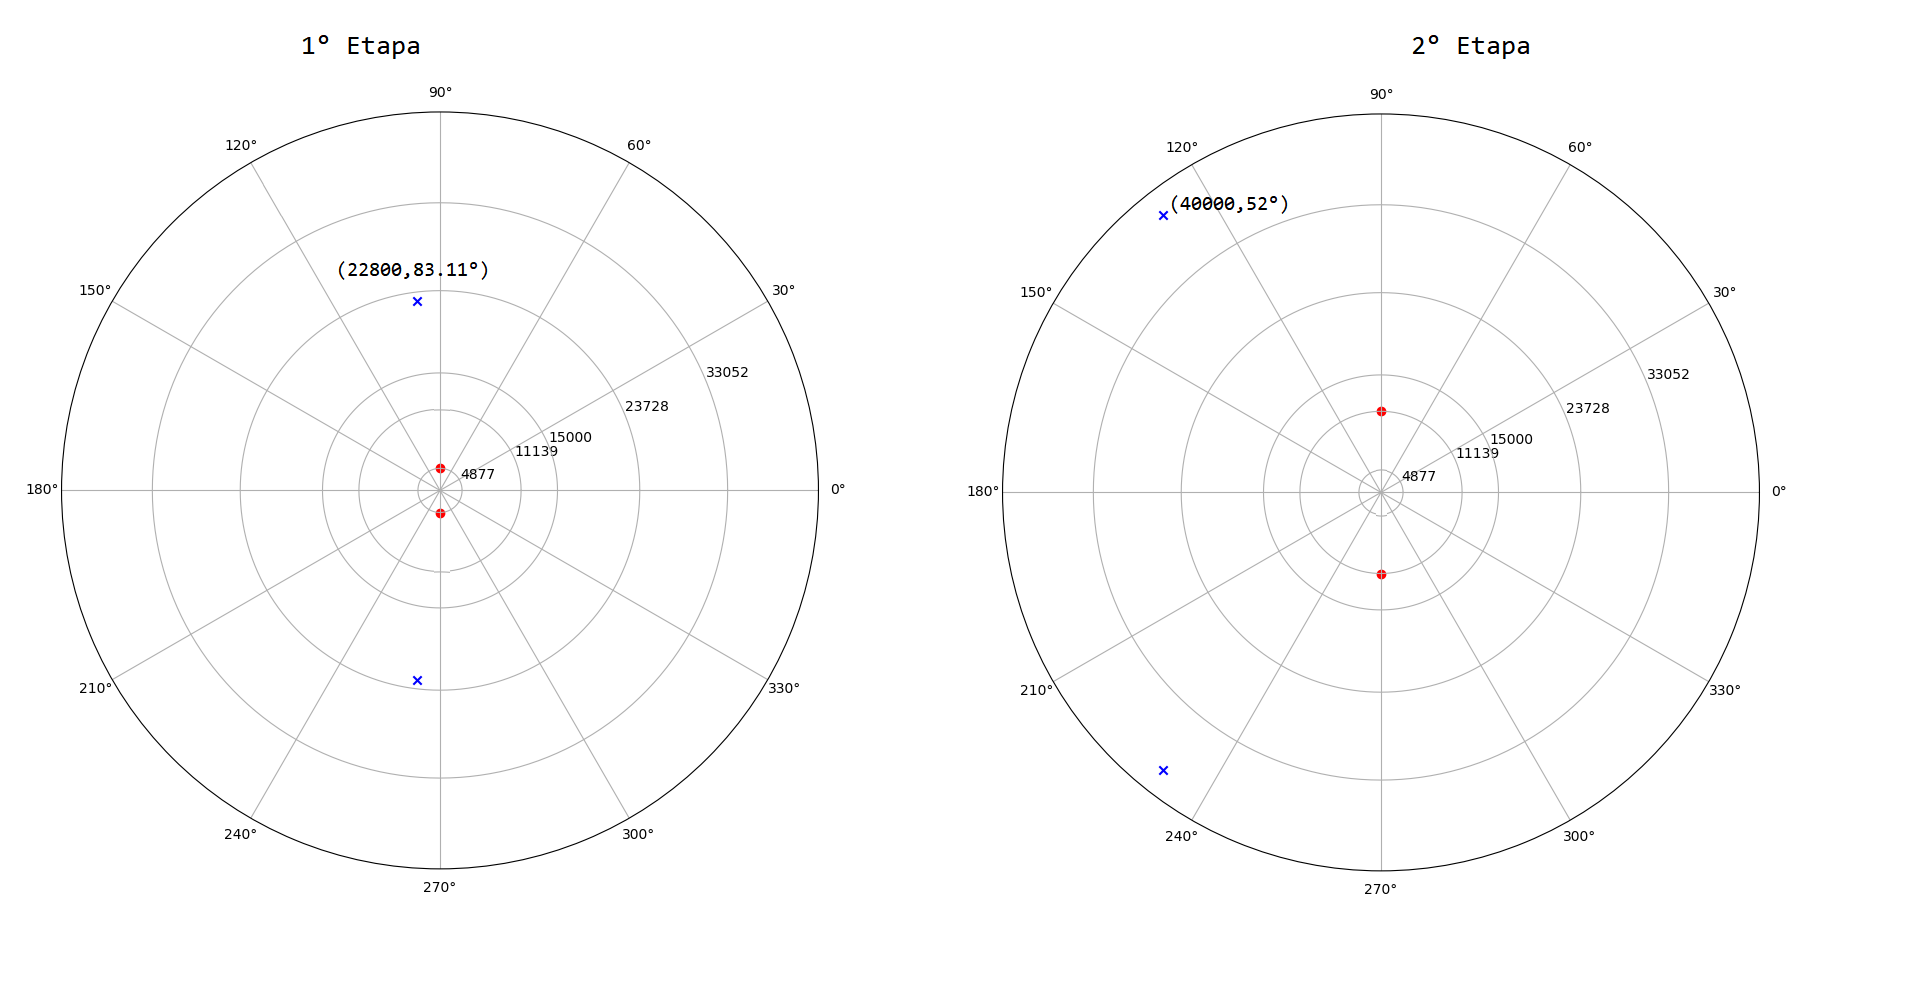
\includegraphics[width=\textwidth]{Imagenes-Ej3/UnionCeros.png}
	\label{fig:CeroPoleUnion}
	\caption{Diagrama Polos y Ceros para cada etapa}
\end{figure}

Luego se decidió colocar la etapa de mayor Q al final.


\subsection{Celda Sedra-Ghorab-Martin.}
La celda Sedra-Ghorab-Martin fue propuesta en el paper ``Optimum Configurations for Single Amplifiers Biquadratic Filters'' como un diseño que permite con un único amplificador operacional (Por eso son llamados Single-Amplifier-Biquad), sintetizar celdas de segundo orden con Q relativamente altos, es destacable que este diseño tiene una baja sensibilidad del Q respecto de la gananica a lazo abierto del amplificador operacional. Este beneficio de la reducción de la sensibilidad del $A_0$, trae un aumento en la sensibilidad respecto a otros componentes pasivos. Originalmente esta celda fue propuesta como una mejora de la celda Deliyannis.
Finalmente en el paper discutido se tomó la configuración de HPB dado a que es lo único que utlizaremos, siendo este el circuito propuesto por el paper.
\begin{figure}[H]
	\centering
	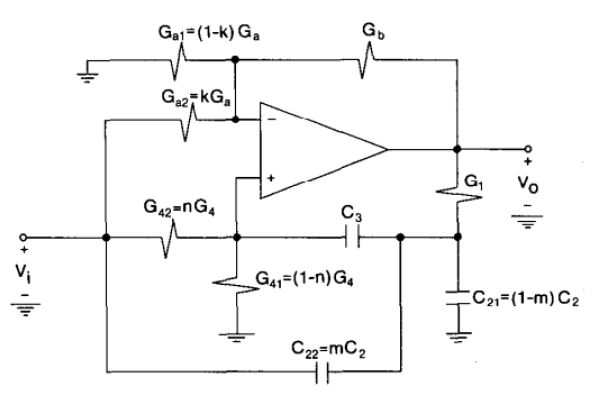
\includegraphics[width=0.5\textwidth]{Imagenes-Ej3/HPBSedra.PNG}
	\label{fig:HPBSedra}
	\caption{Circuito celda SGB-HPB}
\end{figure}
\subsubsection{Cálculo Analítico}
---

\subsubsection{Elecciones de diseño}
Cada una de las funciones transferencia descriptas en (\ref{eq:trans})
 se pueden expresar de la siguiente manera:
\begin{align}
	H_i(s)=\frac{G_\infty (s^2+\omega_z^2)}{s^2+\frac{\omega_0 \cdot s}{Q}+\omega_0^2}
\end{align} 

Luego se siguió con el análisis matemático desarrollado en el paper ``Optimum Configurations for Single Amplifiers Biquadratic Filters''.
De allí se ve la necesidad de introducir algunos parámetros los cuales permiten el diseño de la celda, siendo estos $G_\infty$ el cual es la ganancia cuando $\omega \rightarrow \infty$ , K y $Q_0$ siendo esta ultima una constante que debe cumplir la condición $Q_0 < Q$ permite ajustar el valor de los componentes así queda nominal.  luego se definen los siguientes parámetros. 
\begin{align}
k=\frac{G_\infty\cdot \left(\frac{\omega_z}{\omega_0} \right)^2}{1-\frac{Q_0}{Q}}\\
K=1+\frac{1-\frac{Q_0}{Q}}{2\cdot Q_0^2}\\
n= k\cdot (1-\frac{Q_0 }{K\cdot Q})\\
m=  \left( k-\frac{k}{K} \right) \cdot \left(1+2\cdot \left(\frac{Q_0\cdot \omega_0}{\omega_z}\right)^2 \right)  
\end{align}

A partir de aquí asignando valores para $Q_0$ , C y $R_b$, permite obtener los valores para el resto de las variables con estas equivalencias.  
\begin{align}
	R_a= \frac{1}{(K-1) R_b}\\
	R_{a1}=\frac{1}{(1-k)\cdot R_a}\\
	R_{a2}=\frac{1}{k \cdot R_a}\\
	R_{41}=	\frac{1}{(1-n)\cdot R_4}\\
	R_{42}=	\frac{1}{n\cdot R_4}\\
	C_{21} = (1-m) \cdot C\\
	C_{22} = m \cdot C\\
\end{align}
El análisis de sensibilidades que se obtiene del circuito, el cual coincide con lo publicado en el paper es la siguiente: 
\begin{table}[H]
\centering
\begin{tabular}{ccc}
Componente & $S^\omega_0$ & $S^Q$                                      \\ \hline
$S_{R_1}$  & -0.5         & $-\left( \frac{Q}{Q_0} -0.5 \right)$       \\
$S_{C}$    & -0.5         & $0.5\cdot \left( \frac{Q}{Q_0} -1 \right)$ \\
$S_{R_4}$  & -0.5         & $\left( \frac{Q}{Q_0} -0.5 \right)$        \\
$S_{R_a}$  & 0            & $-\left( \frac{Q}{Q_0} -1 \right)$         \\
$S_{R_b}$  & 0            & $\left( \frac{Q}{Q_0} -1 \right)$         
\end{tabular}
\end{table}


En base a esta tabla se tomo especial cuidado en la elección de componentes y en el matcheo de impedancias.

Se tomaron como valor de los componentes los presentados en la siguiente tabla:
\begin{table}[H]
\centering
\begin{tabular}{ccccc}
\multicolumn{1}{c}{Componente} & \multicolumn{1}{c}{1er Etapa} & \multicolumn{1}{c}{Composición} & 2da Etapa        & Composición            \\ \hline
$R_{a1}$                          & 12.36k $\Omega$               & 330+12k $\Omega$                & 6.2k $\Omega$    & 1.5k + 4.7k $\Omega$   \\
$R_{a2}$                          & 100k $\Omega$                 & 100k $\Omega$                   & 89.67 k $\Omega$ & 22k + 68k $\Omega$     \\
$R_b$                          & 50.72 k $\Omega$              & 3.9k + 47k $\Omega$             & 1k$\Omega$       & 1k$\Omega$             \\
$R_{41}$                          & 23.88k $\Omega$               & 1.8k+22k $\Omega$               & 203.36k $\Omega$ & 270k // 820 k $\Omega$ \\
$R_{42}$                          & 207k $\Omega$                 & 27k + 180k $\Omega$             & 4.19 M$\Omega$   & 1.8M + 2.2M $\Omega$   \\
$R_1$                          & 74.05k $\Omega$               & 18k + 56k $\Omega$              & 25.07k $\Omega$  & 10k+15k $\Omega$       \\
$C_3$                          & 100 pF                        & 100 pF                          & 100 pF           & 100 pF                 \\
$C_{21}$                          & 74.14 pF                      & 18p // 56p F                    & 18.52p F         & 22pF + 120pF           \\
$C_{22}$                          & 25.86pF                       & 33p + 120p F                    & 81.48pF          & 82pF+12nF             
\end{tabular}
\end{table}


Se calculó el error porcentual asociado a la aproximación de la resistencias viéndose en la siguiente tabla.
\begin{table}[H]
\centering
\begin{tabular}{lll}
\multicolumn{1}{c}{Error Porcentual} & \multicolumn{1}{c}{1er Etapa} & \multicolumn{1}{c}{2da Etapa} \\ \hline
$R_{a1}$                                & 0.2 $\%$                      & $\approx 0 \%$                \\
$R_{a2}$                                & $\approx 0 \%$                & 0.4 $\%$                      \\
$R_b$                                & 0.4 $\%$                      & $\approx 0 \%$                \\
$R_{41}$                                & 0.3 $\%$                      & 0.1 $\%$                      \\
$R_{42}$                                & $\approx 0 \%$                & 0.3 $\%$                      \\
$R_1$                                & 0.1 $\%$                      & 0.3 $\%$                      \\
$C_3$                                & $\approx 0 \%$                & $\approx 0 \%$                \\
$C_{21}$                                & 0.2 $\%$                      & 0.4 $\%$                      \\
$C_{22}$                                & 0.1 $\%$                      & 0.1 $\%$                     
\end{tabular}
\end{table}

Un criterio utilizado fue tomar capacitores pequeños dado a que ellos son mas certeros y no varían tanto frente a la temperatura.  

\subsubsection{Acoplamiento de Impedancias.}
Para que ambas etapas no se carguen entre si la impedancia de entrada de la segunda etapa debe ser mucho mayor a la de salida de la primera.
Así se simuló la impedancia de entrada de ambas etapas obteniendo las siguientes gráficas:
\begin{figure}[H]
	\centering
	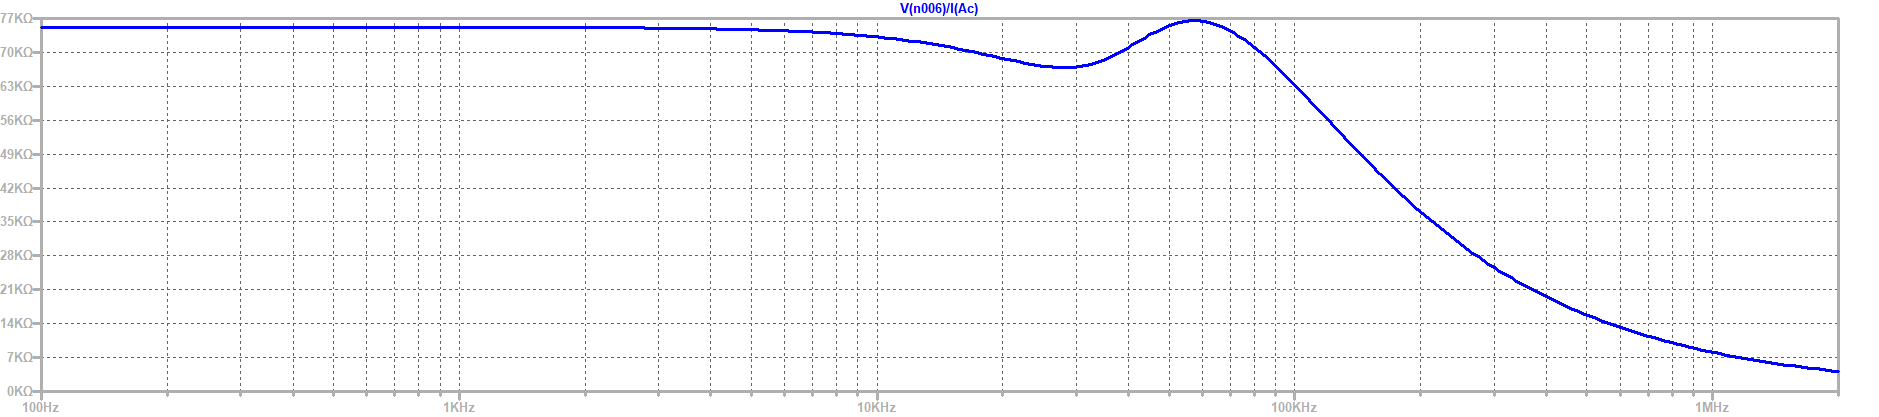
\includegraphics[width=\textwidth]{Imagenes-Ej3/ZinE1.png}
	\label{fig:zine1}
	\caption{Impedancia de entrada 1ra etapa}
\end{figure}

\begin{figure}[H]
	\centering
	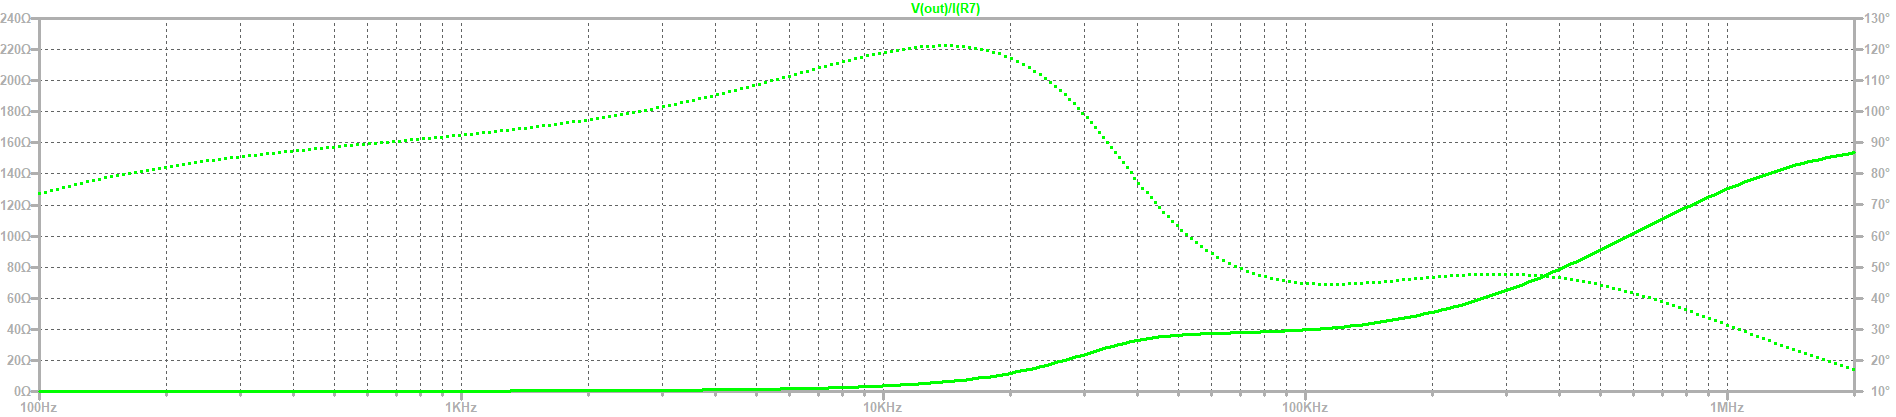
\includegraphics[width=\textwidth]{Imagenes-Ej3/ZoutE1.png}
	\label{fig:zoute1}
	\caption{Impedancia de salida 1ra etapa}
\end{figure}

\begin{figure}[H]
	\centering
	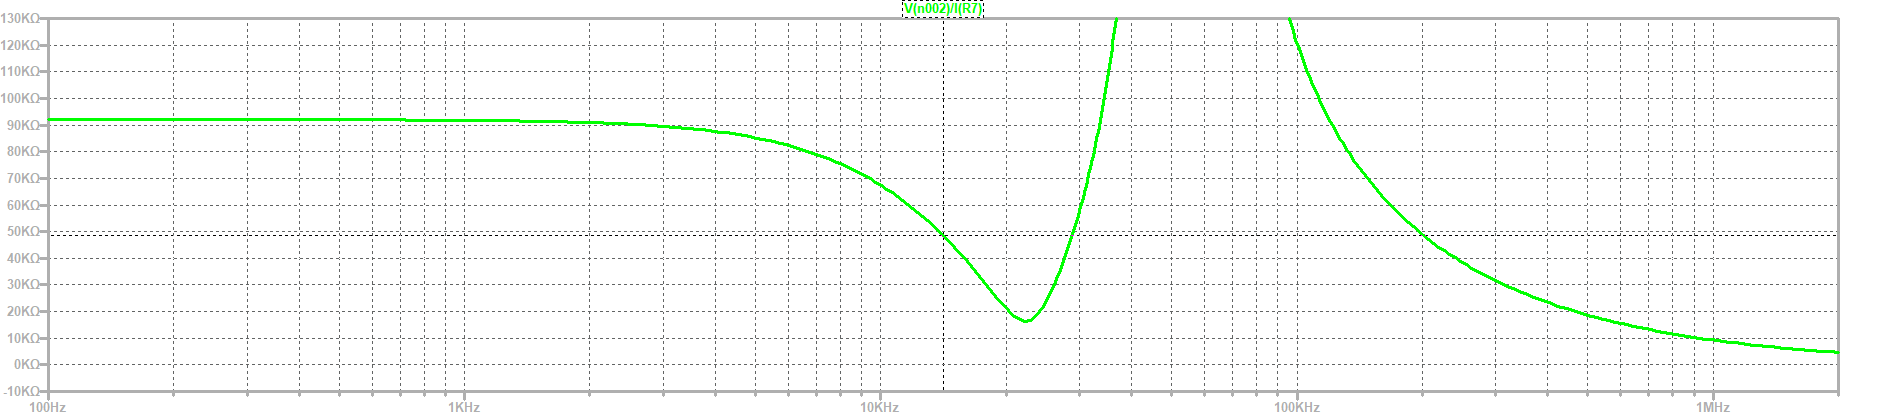
\includegraphics[width=\textwidth]{Imagenes-Ej3/ZinE2.png}
	\label{fig:zine2}
	\caption{Impedancia de entrada 2da etapa}
\end{figure}
Se puede concluir luego de estas gráficas que el acoplamiento de impedancias se dará.
\subsection{Respuesta en Frecuencia.}
Se realizó un análisis de Montecarlo a la respuesta en frecuencia del circuito, utilizando una tolerancia de las resistencias al 1$\%$ y capacitores al 10$\%$ obteniendo la siguiente dispersión
\begin{figure}[H]
	\centering
	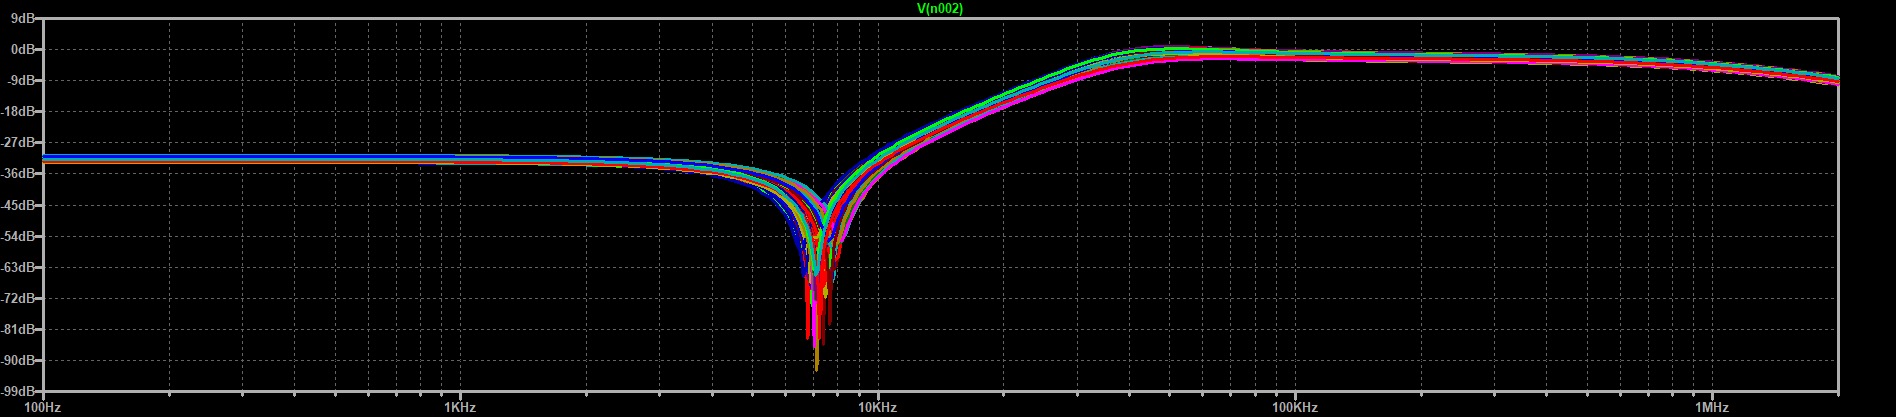
\includegraphics[width=\textwidth]{Imagenes-Ej3/mcsedra.png}
	\label{fig:mcsedra}
	\caption{Análisis de Montecarlo Filtro entero.}
\end{figure}
Se puede apreciar una dispersión en la frecuencia de corte del sistema, a causa de esto se tuvo en cuenta en el diseño utilizar un preset el cual tenga sensibilidad con este con el propósito de poder ajustarlo, un problema con esta metodología es que no solamente importa la ubicación del cero de transmisión sino también su Q, una solución a esta problemática fue utilizar un preset en cada etapa, donde en la primer etapa el preset sería colocado sobre $R_1$ dado a la sensibilidad del $\omega_z$ para con el, y un preset en la segunda etapa (la de mayor Q) en la resistencia  $R_b$, finalmente se midió el circuito previo a la colocación de los presets, y el mismo cumplía con las especificaciones, por lo tanto se tomo la decisión de no utilizar un preset. 
\subsubsection{Etapas.}
Además de el montecarlo de el filtro en su totalidad de realizó un análisis de montecarlo para cada etapa por separado.
\begin{figure}[H]
	\centering
	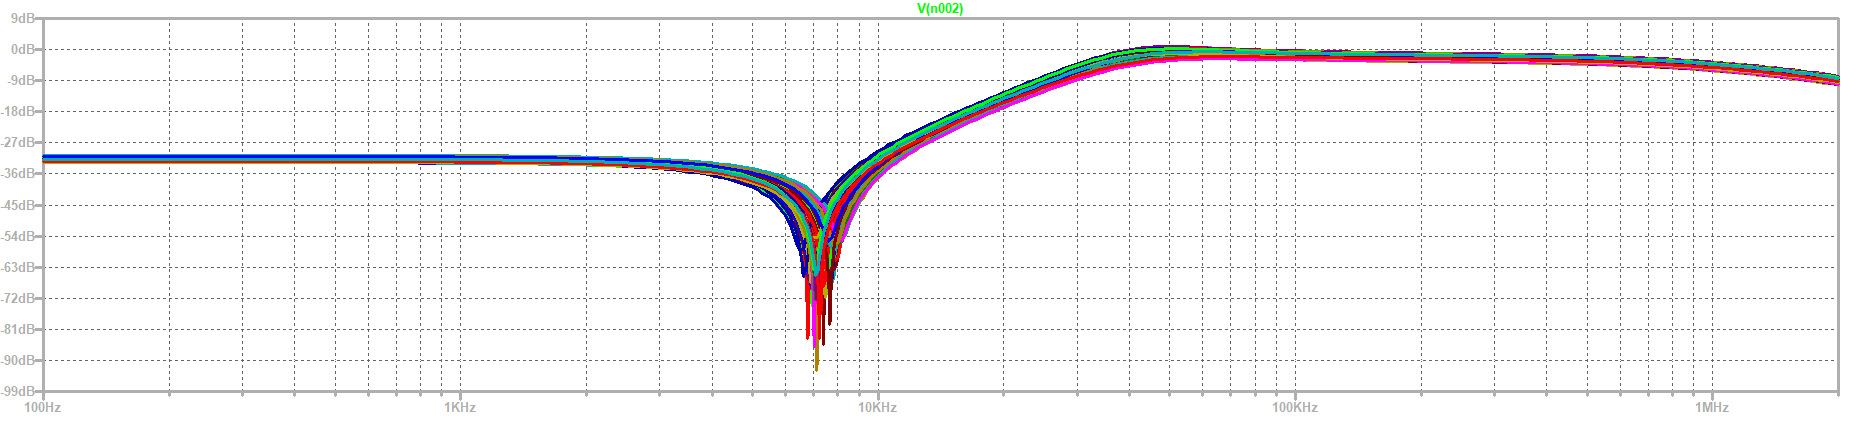
\includegraphics[width=\textwidth]{Imagenes-Ej3/mcsedraE1.png}
	\label{fig:mcsedrae1}
	\caption{Análisis de Montecarlo primer etapa.}
\end{figure}
En esta imagen se puede observar como la dispersion de la primer etapa modifica seriamente el Q tanto como la posición del cero de transmisión.
\begin{figure}[H]
	\centering
	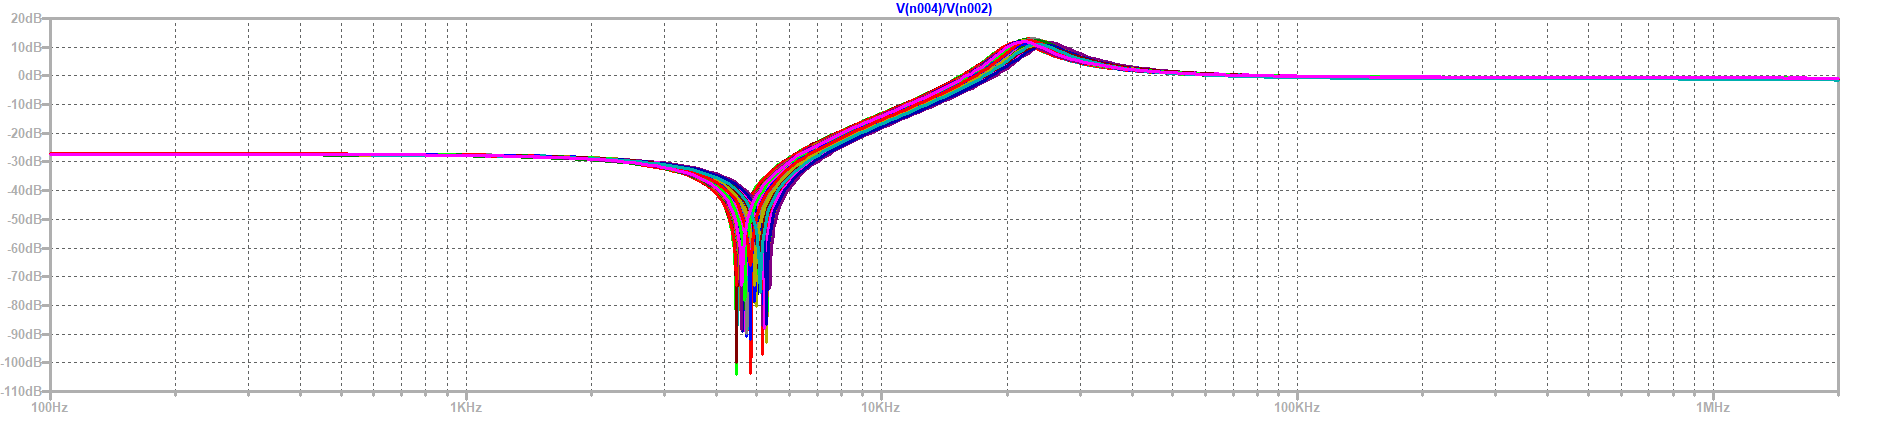
\includegraphics[width=\textwidth]{Imagenes-Ej3/mcsedraE2.png}
	\caption{Análisis de Montecarlo segunda etapa.}
	\label{fig:mcsedrae2}
\end{figure}
Algo que se puede apreciar en la figura ( \ref{fig:mcsedrae2} ) es que dependiendo en cual de las variaciones se encuentre el circuito, corresponderá directamente con la altura del sobrepico que habrá, aparte de su correspondietne cero, si bien para ambas simulaciones los valores de la transferencia para $s\rightarrow 0$ y $s\rightarrow \infty$ son aproximadamente constantes mas allá de la dispersión.

Además se hicieron simulaciones de como el preset podría ser utilizado para variar el Q del circuito.

Comenzando por utilizar un preset en la primer etapa sobre $R_1$.
\begin{figure}[H]
	\centering
	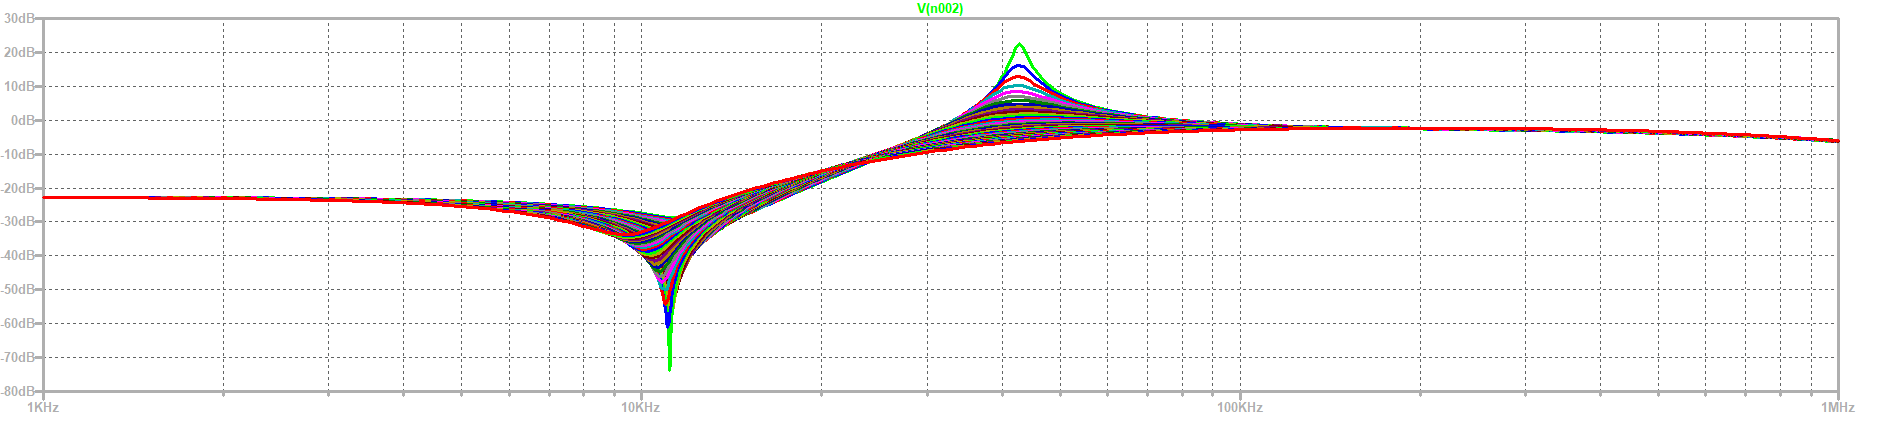
\includegraphics[width=\textwidth]{Imagenes-Ej3/mcPoteR6E1.png}
	\label{fig:presete1}
	\caption{Análisis uso de preset primer etapa.}
\end{figure}
De aqui se puede concluir que la utilización de un preset en esta etapa ayuda a fijar tanto a fijar un Q como a ajustar el cero de transmisión.

Luego se prosiguió por la utilización de un preset en la segunda etapa, sobre la resistencia $R_b$:
\begin{figure}[H]
	\centering
	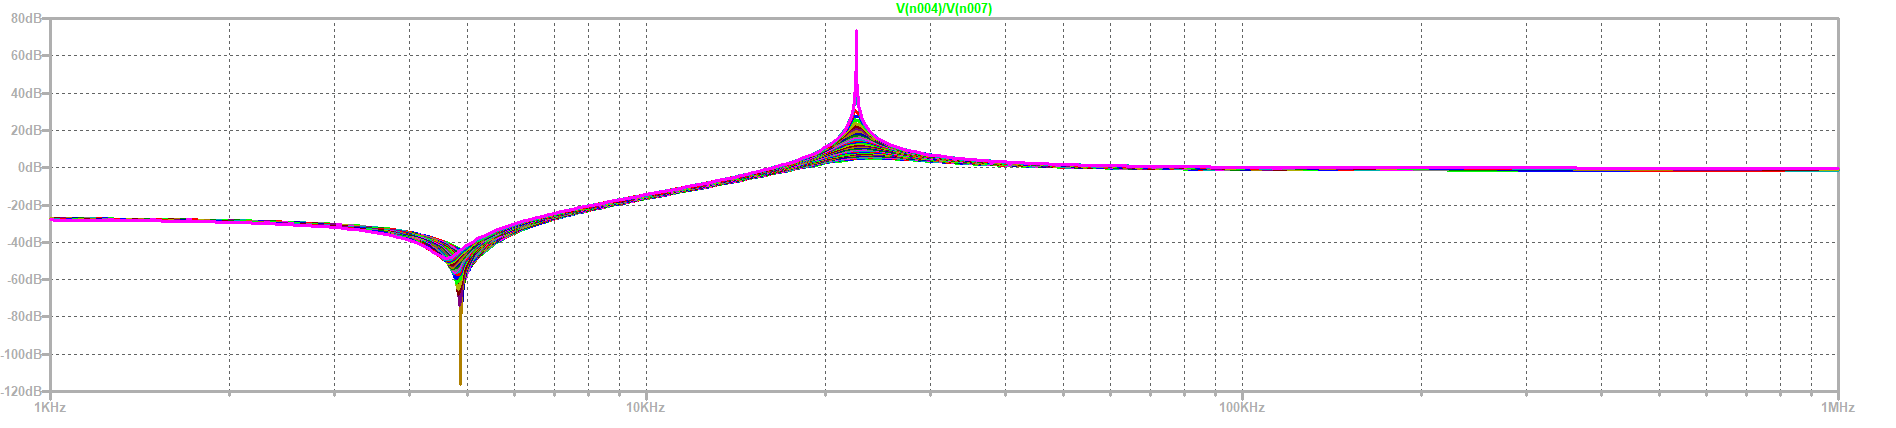
\includegraphics[width=\textwidth]{Imagenes-Ej3/mcPoteR3E2.png}
	\label{fig:presete2}
	\caption{Análisis uso de preset segunda etapa.}
\end{figure}
 De aquí, como era esperado, se ve que tiene una mayor sensibilidad respecto al Q lo cual sería el preset ideal para ajustarlo.

Finalmente dado a que inicialmente se realizó el filtro y cumplía las especificaciones se decidió no utilizar un preset, sin embargo se tuvo la precaución de diseñar una etapa de compensación de ganancia para el caso en el que la variación de las condiciones ambientales modifique el filtro y esta sea necesaria, esta etapa consiste en un no inversor con ganancia variable.

\subsubsection{Filtro definitivo.}
Se realizó el filtro obteniendo la siguiente respuesta en frecuencia 
\begin{figure}[H]
	\centering
	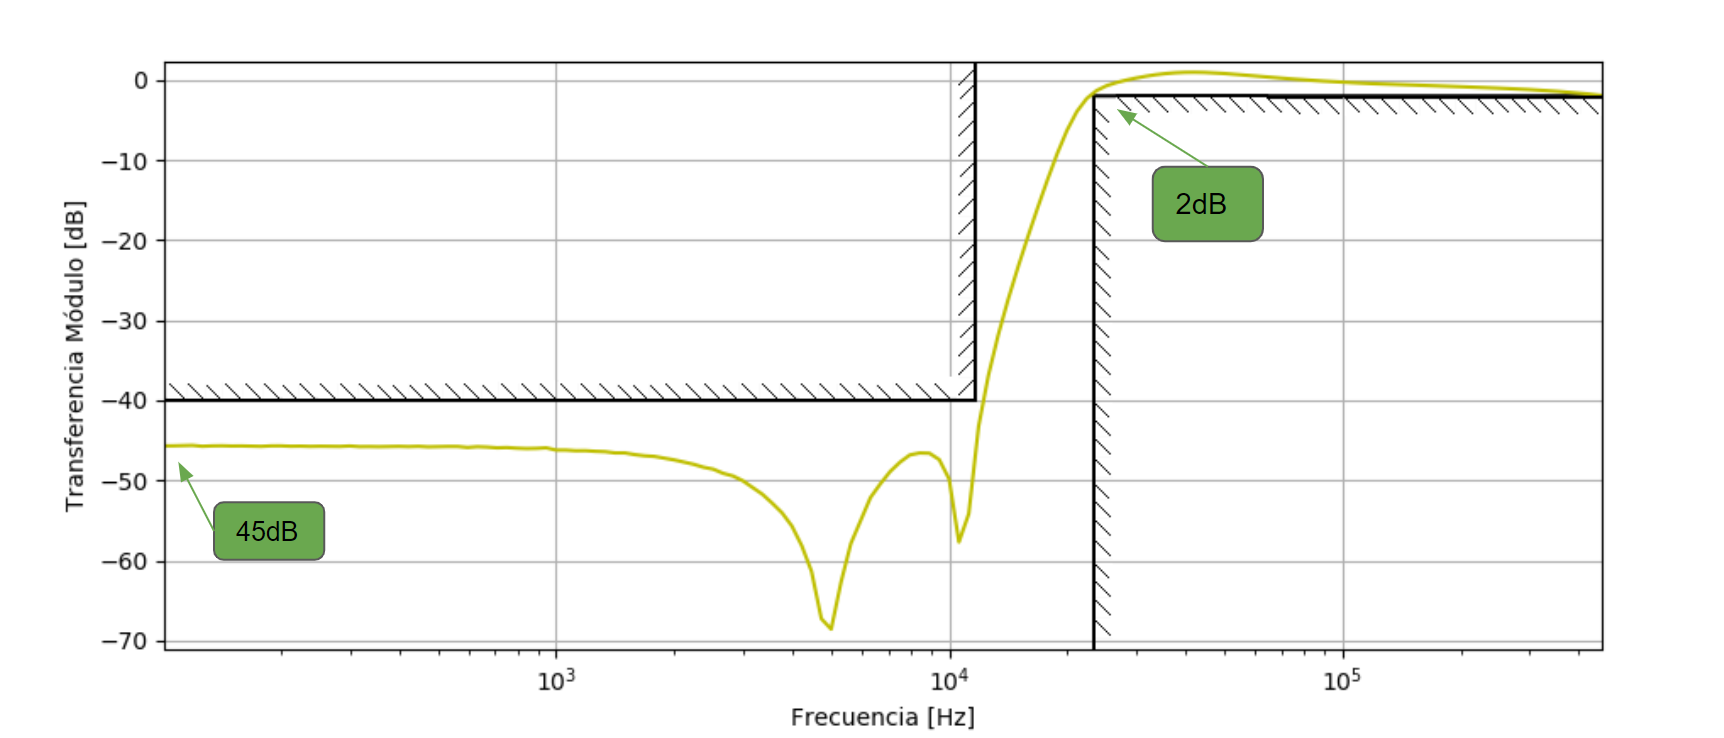
\includegraphics[width=\textwidth]{Imagenes-Ej3/BodeSedra.png}
	\label{fig:BodeSedra}
	\caption{Filtro High-Pass Módulo}
\end{figure}
\begin{figure}[H]
	\centering
	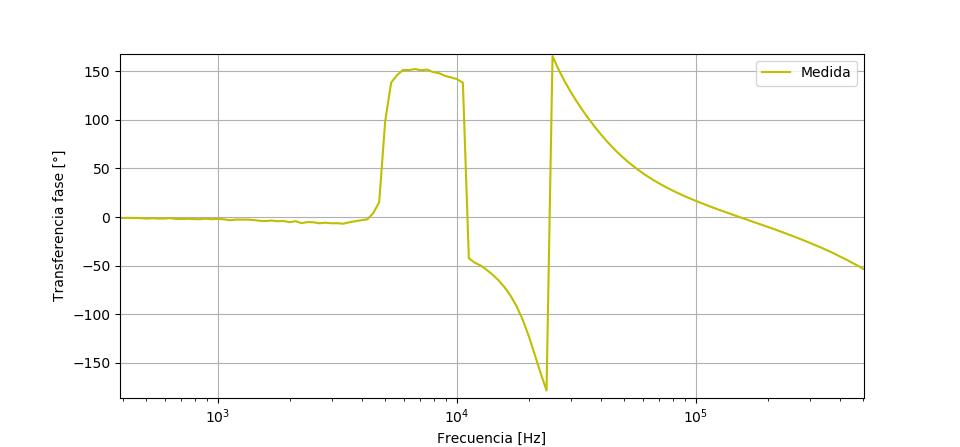
\includegraphics[width=\textwidth]{Imagenes-Ej3/FaseBodeSedra.png}
	\label{fig:FaseBodeSedra}
	\caption{Filtro High-Pass Fase}
\end{figure}
Es de valor apreciar el hecho de que se cumple la plantilla.


También puede tomarse en cuenta que los resultados obtenidos se corresponden con lo simulado y calculado:

\begin{figure}[H]
	\centering
	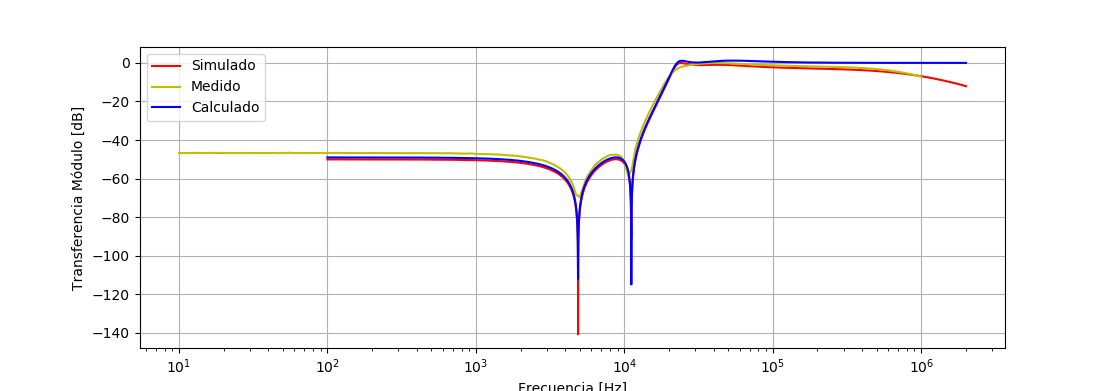
\includegraphics[width=\textwidth]{Imagenes-Ej3/BodeMedCalcSim.png}
	\label{fig:BodeSedraComp}
	\caption{Filtro High-Pass Módulo comparación.}
\end{figure}
\begin{figure}[H]
	\centering
	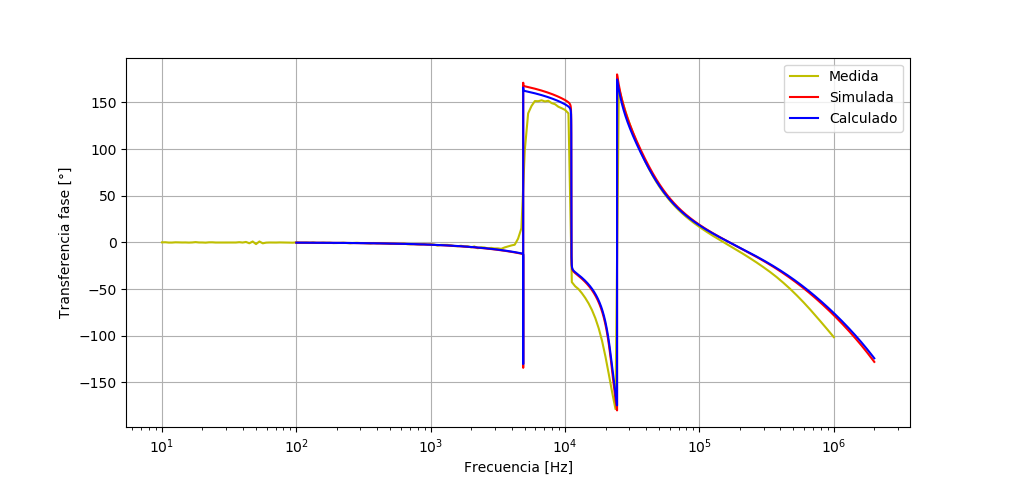
\includegraphics[width=\textwidth]{Imagenes-Ej3/BodeMedCalcSimFase.png}
	\label{fig:FaseBodeSedraComp}
	\caption{Filtro High-Pass Fase comparación.}
\end{figure}
\subsection{Rango Dinámico.}
\begin{Huge}
???????????????????????????????????????????????
\end{Huge}
\subsection{Estabilidad.}
Se intentó en esta sección lograr que la celda oscile, introduciéndole una cuadrada la cual es sabido esta compuesta por un gran numero de frecuencias, así también variando no solo la amplitud de la misma sino también su frecuencia y duty-cycle, sin poder hacer oscilar a la celda. La siguiente imagen es la respuesta de la celda al escalón.
\begin{figure}[H]
	\centering
	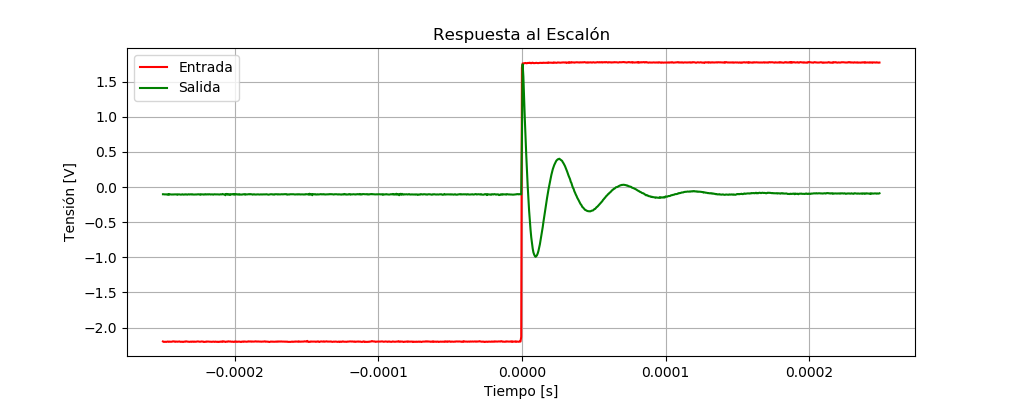
\includegraphics[width=\textwidth]{Imagenes-Ej3/Step.png}
	\label{fig:stepresponse}
	\caption{Respuesta al escalón}
\end{figure}
\subsection{Conclusiones}
La celda sedra es una gran alternativa cuando no se tiene un amplificador operacional con una ganancia a lazo abierto relativamente estable, también permite la implementación de un filtro de segundo orden con tan solo 1 operacional, mientras que por ejemplo la celda universal utiliza 3 de ellos, también tiene el beneficio de poder sintetizar valores de Q relativamente altos gracias a su doble realimentación tanto negativa como positiva, dando esta ultima una de sus desventajas que es la posibilidad de que haya una oscilación en el circuito.
%
%\begin{figure}[H]
%	\centering
%	\includegraphics[width=0.4\textwidth]{/ImagenesEjercicio3/Graph.png}
%	\label{fig:graph}
%\end{figure}

\end{document}